\chapter{Конструкторская часть}

В данном разделе разработаны схемы реализаций алгоритма поиска всех вхождений подстроки в файле с учетом опечаток.

\section{Требования к программному обеспечению}

К программе предъявлены ряд требований:

\begin{itemize}[label=---]
	\item должен присутствовать интерфейс для выбора действий;
	\item должна работать с нативными потоками;
\end{itemize}

\section{Разработка алгоритмов}

На рисунках \ref{fig:parallel} -- \ref{fig:prefix} приведены схемы многопоточной реализации алгоритма поиска подстроки в файле с учетом опечаток.

\begin{figure}[h]
	\centering
	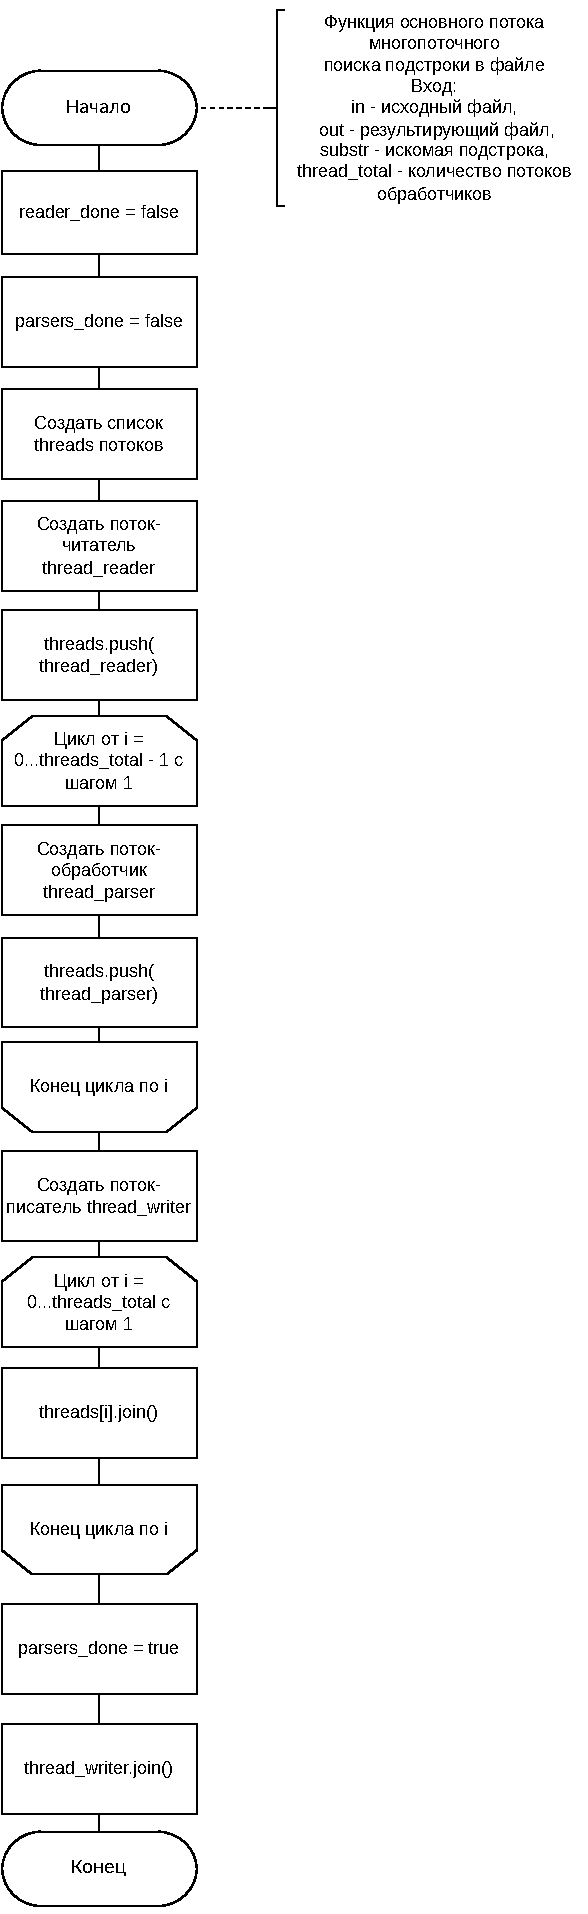
\includegraphics[height=0.9\textheight]{img/threads_main.pdf}
	\caption{Схема алгоритма работы основного потока, запускающего вспомогательные потоки.}
	\label{fig:parallel}
\end{figure}

\clearpage

\begin{figure}[h]
	\centering
	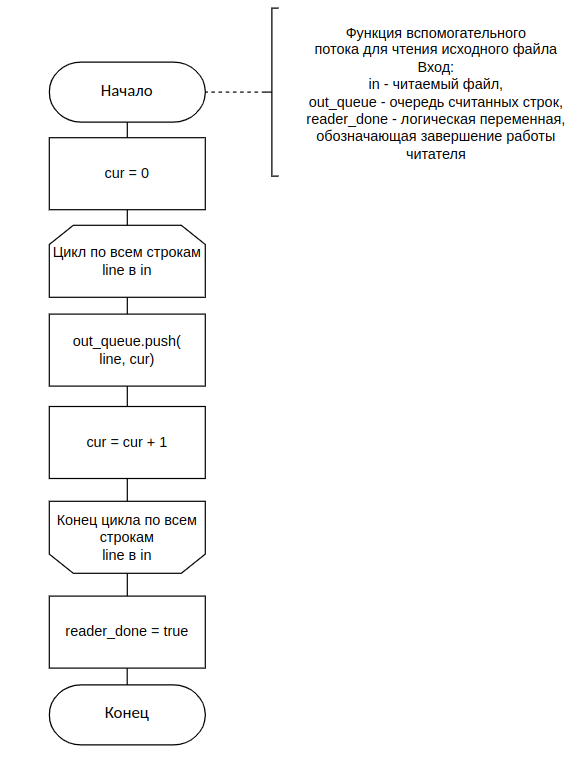
\includegraphics[height=0.8\textheight]{img/thread_reader.png}
	\caption{Схема алгоритма работы потока, выполняющего чтение из файла.}
	\label{fig:thread_reader}
\end{figure}

\clearpage

\begin{figure}[h]
	\centering
	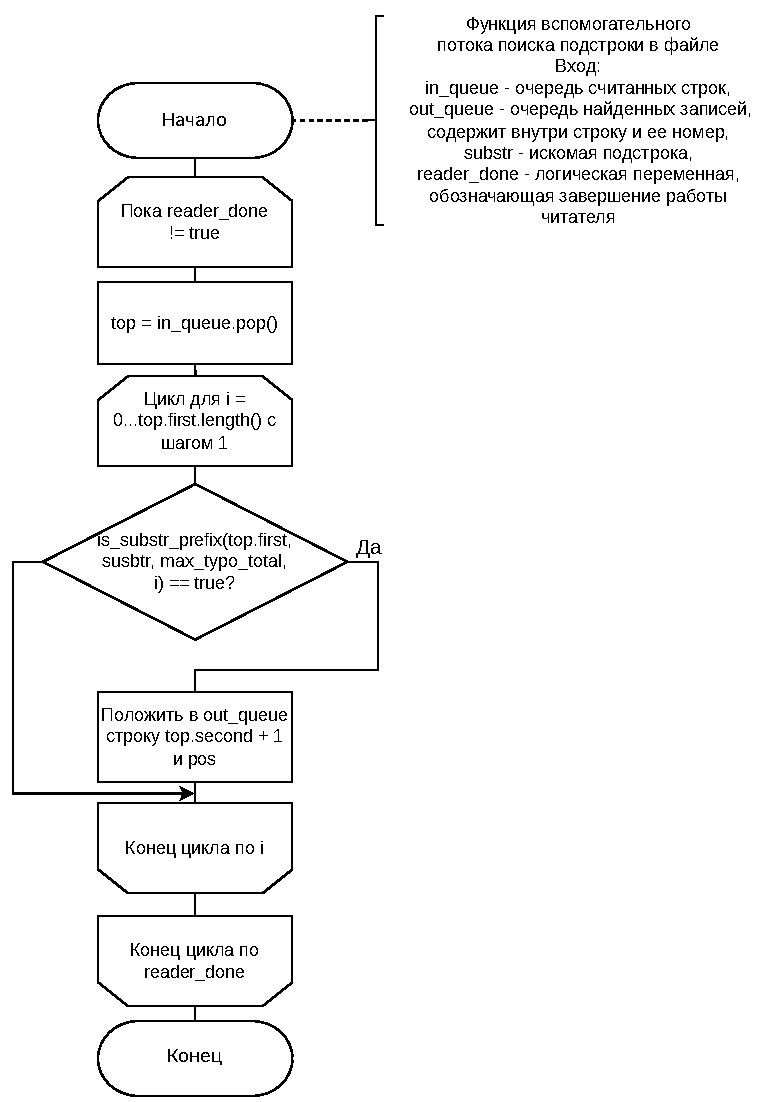
\includegraphics[height=0.8\textheight]{img/thread_substr.pdf}
	\caption{Схема алгоритма работы потока, обрабатывающего считанные строки.}
	\label{fig:parser}
\end{figure}

\clearpage

\begin{figure}[h]
	\centering
	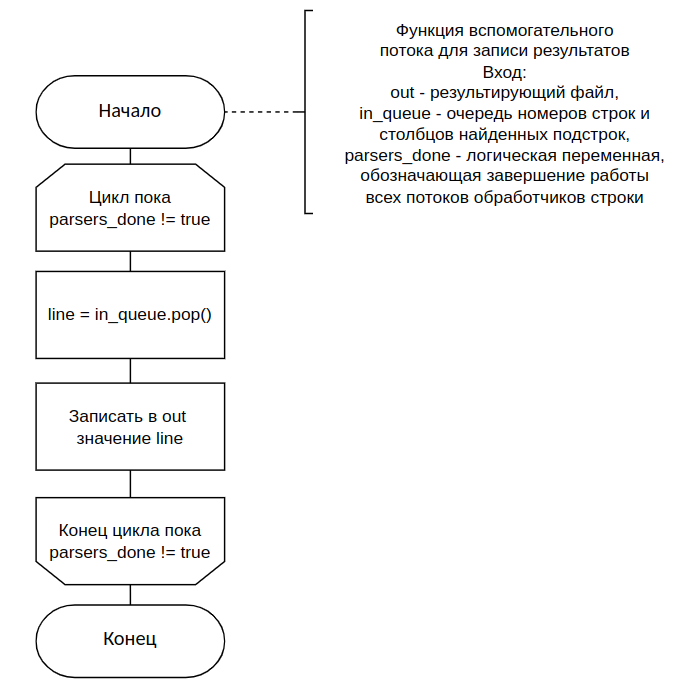
\includegraphics[height=0.6\textheight]{img/thread_writer.png}
	\caption{Схема алгоритма работы потока, записывающего результаты в файл.}
	\label{fig:writer}
\end{figure}

\clearpage

\begin{figure}[h]
	\centering
	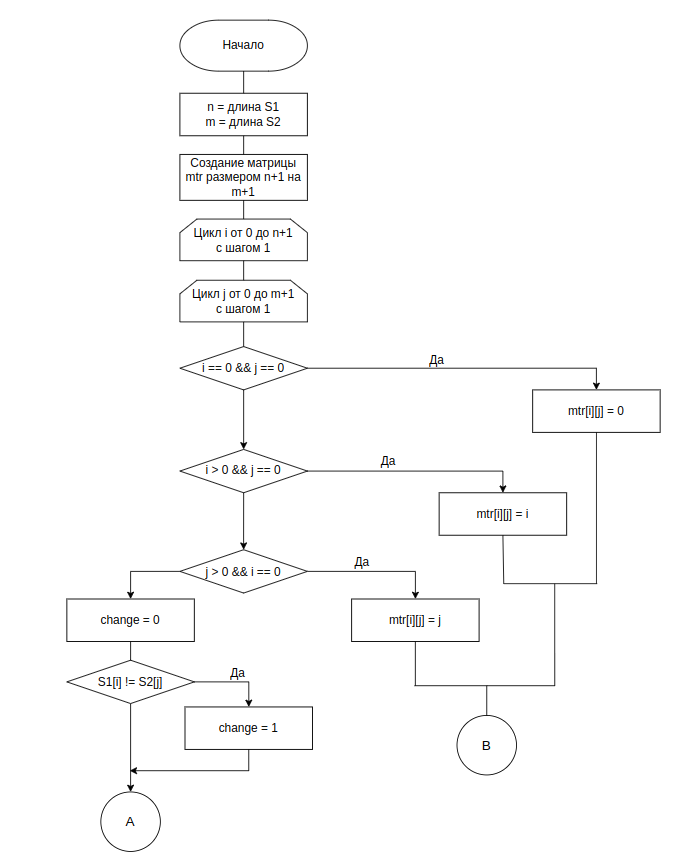
\includegraphics[width=\textwidth]{img/dliter1.png}
	\caption{Схема 1 нерекурсивного алгоритма нахождения расстояния Дамерау-Левенштейна}
	\label{fig:DLiter1}
\end{figure}

\clearpage

\begin{figure}[h]
	\centering
	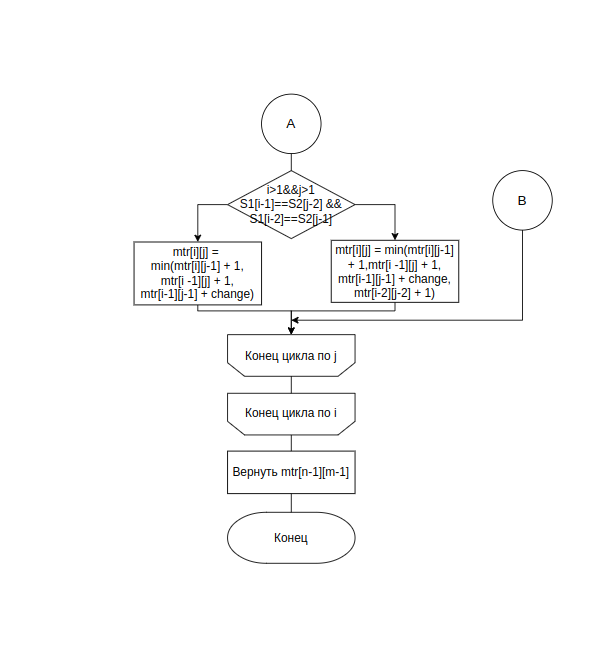
\includegraphics[width=\textwidth]{img/dliter2.png}
	\caption{Схема 2 нерекурсивного алгоритма нахождения расстояния Дамерау-Левенштейна}
	\label{fig:DLiter2}
\end{figure}

\clearpage

\begin{figure}[h]
	\centering
	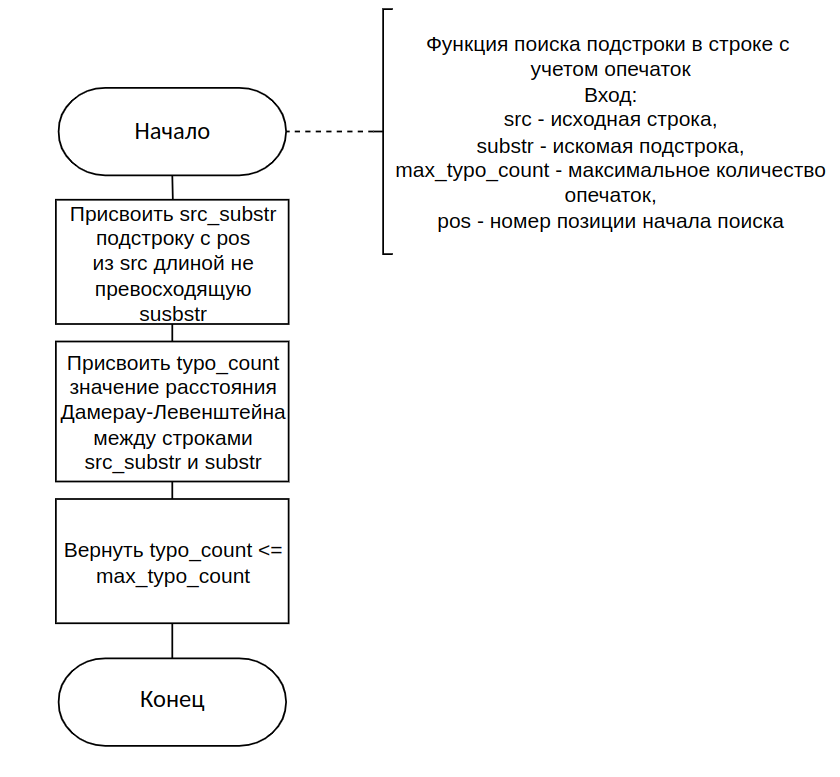
\includegraphics[width=\textwidth]{img/prefix.png}
	\caption{Схема функции нахождения подстроки с учетом опечаток}
	\label{fig:prefix}
\end{figure}

\clearpage

\section*{Вывод}

В данном разделе разработаны схемы реализаций рассматриваемого алгоритма.
